% A simple Tree
% Author: Stefan Kottwitz
% https://www.packtpub.com/hardware-and-creative/latex-cookbook
\documentclass[border=10pt]{standalone}
\usepackage{tikz}
\begin{document}
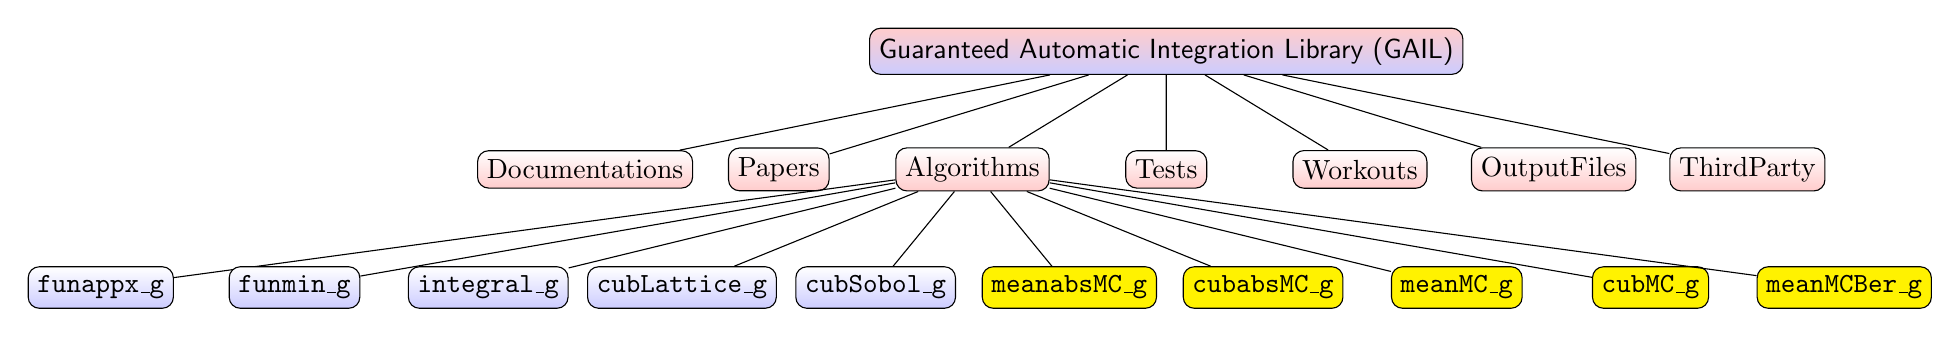
\begin{tikzpicture}[sibling distance=7em,
%%  every node/.style = {shape=rectangle, rounded corners,
%    draw, align=center,
%    top color=white, bottom color=blue!20}]]
  every node/.style = {shape=rectangle, rounded corners,
    draw, align=center}]]
  \node[top color=red!20, bottom color=blue!20, font = \sffamily] {Guaranteed Automatic Integration Library (GAIL)}
    child { node[top color=white, bottom color=red!20] {Documentations} }
  child { node[top color=white, bottom color=red!20] {Papers} }
   child { node [top color=white, bottom color=red!20]{Algorithms}
      child { node[top color=white, bottom color=blue!20] {{\tt funappx\_g}}}
      child { node[top color=white, bottom color=blue!20] {{\tt funmin\_g}}}
               child { node[top color=white, bottom color=blue!20] {{\tt integral\_g}}}
            child { node[top color=white, bottom color=blue!20] {{\tt cubLattice\_g}}}
                  child { node[top color=white, bottom color=blue!20] {{\tt cubSobol\_g}}}
      child { node[fill = yellow] {{\tt meanabsMC\_g}}}
      child { node[fill = yellow] {{\tt cubabsMC\_g}}}
         child { node[fill = yellow] {{\tt meanMC\_g}}}
      child { node[fill = yellow] {{\tt cubMC\_g}}}
            child { node[fill = yellow] {{\tt meanMCBer\_g}}}}
child { node[top color=white, bottom color=red!20] {Tests} }
            child { node[top color=white, bottom color=red!20] {Workouts} }
                child { node[top color=white, bottom color=red!20] {OutputFiles} }
                                child { node[top color=white, bottom color=red!20] {ThirdParty} };
\end{tikzpicture}
\end{document}